% Figure from MATH 493 notes, section 56 (the five possible squares, with pipes). Added, not from lecture (after WS 12).
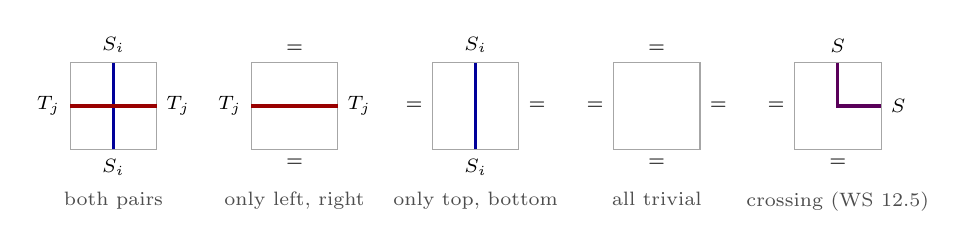
\begin{tikzpicture}[font=\scriptsize, x=1cm, y=1cm]
  \def\sq#1{\draw[gray!70] (#1,0) rectangle ++(1.1,1.1);}
  \sq{0} \node[above] at (0.55,1.1) {$S_i$}; \node[below] at (0.55,0) {$S_i$}; \node[left] at (0,0.55) {$T_j$}; \node[right] at (1.1,0.55) {$T_j$};
  \draw[very thick, blue!60!black] (0.55,0) -- (0.55,1.1); \draw[very thick, red!60!black] (0,0.55) -- (1.1,0.55);
  \sq{2.3} \node[above] at (2.85,1.1) {$=$}; \node[below] at (2.85,0) {$=$}; \node[left] at (2.3,0.55) {$T_j$}; \node[right] at (3.4,0.55) {$T_j$};
  \draw[very thick, red!60!black] (2.3,0.55) -- (3.4,0.55);
  \sq{4.6} \node[above] at (5.15,1.1) {$S_i$}; \node[below] at (5.15,0) {$S_i$}; \node[left] at (4.6,0.55) {$=$}; \node[right] at (5.7,0.55) {$=$};
  \draw[very thick, blue!60!black] (5.15,0) -- (5.15,1.1);
  \sq{6.9} \node[above] at (7.45,1.1) {$=$}; \node[below] at (7.45,0) {$=$}; \node[left] at (6.9,0.55) {$=$}; \node[right] at (8.0,0.55) {$=$};
  \sq{9.2} \node[above] at (9.75,1.1) {$S$}; \node[below] at (9.75,0) {$=$}; \node[left] at (9.2,0.55) {$=$}; \node[right] at (10.3,0.55) {$S$};
  \draw[very thick, violet!70!black] (9.75,1.1) -- (9.75,0.55) -- (10.3,0.55);
  \foreach \x/\t in {0.55/{both pairs}, 2.85/{only left, right}, 5.15/{only top, bottom}, 7.45/{all trivial}, 9.75/{crossing (WS 12.5)}} { \node[below=12pt, text=black!70] at (\x,0) {\t}; }
\end{tikzpicture}
